\chapter{Especificación de requisitos}

Este capítulo es una Especificación de Requisitos Software para el software que se va a realizar siguiendo las directrices dadas por el estándar IEEE830 \cite{iee830}.

\section{Introducción}

\subsection{Propósito}

Este capítulo de especificación de requisitos tiene como objetivo definir las especificaciones funcionales y no funcionales para el desarrollo de un software que permitirá visualizar e interactuar con los datos DICOM obtenidos al someter a una escultura a un TAC. Éste software será utilizado principalmente por restauradores.

\subsection{Ámbito del sistema}

En la actualidad los datos DICOM obtenidos tras un TAC se utilizan, principalmente, en el campo donde surgieron, la medicina. No obstante, esto no significa que solo se pueda aplicar ahí. Con este software, llamado \myTitle, se tratará de trasladar esta técnica al campo de la restauración de bienes culturales y poder visualizar e interactuar con los datos DICOM obtenidos con esculturas.

\subsection{Definiciones, acrónimos y abreviaturas}

\begin{itemize}
	\item \textbf{ERS}: Especificación de Requisitos Software.
	\item \textbf{GUI} (\textit{Graphic User Interface}): Interfaz gráfica de usuario.
	\item \textbf{DICOM} (\textit{Digital Imaging and Comunication in Medicine}): Datos de donde se obtienen las imágenes.
	\item \textbf{TAC} (Tomografía Axial Computerizada): Escáner en el que se obtienen los datos DICOM.
	\item \textbf{VTK} (\textit{The Visualization ToolKit}): Librería gráfica que se utilizará.
	\item \textbf{Qt}: Librería que se utilizará para realizar la GUI.
	\item \textbf{Volumen}: Conjunto de datos en los que para cada posición XYZ se tiene un valor determinado.
	\item \textbf{Función de transferencia}: Función utilizada para visualizar los datos deseados de un volumen.
	\item \textbf{Corte}: Vista de la figura a través de un plano. Por ejemplo, al cortar con una sierra un tronco por la mitad, se puede ver cómo es por dentro en esa posición por donde se ha cortado.
	\item \textbf{Widget}: Elemento de la GUI.
\end{itemize}

\subsection{Visión general del documento}

Este capítulo consta de tres secciones:
\begin{itemize}
	\item En la primera sección se realiza una introducción a éste y se proporciona una visión general de la ERS.
	\item En la segunda sección se realiza una descripción general a alto nivel del software, describiendo los factores que afectan al producto y a sus requisitos y con el objetivo de conocer las principales funcionalidades de éste.
	\item En la tercera sección se definen detalladamente los requisitos que deberá satisfacer el software.
\end{itemize}

\section{Descripción general}

\subsection{Perspectiva del producto}

El software \myTitle tiene como objetivo interactuar con datos DICOM, pero no es el encargado de generarlos. Para generarlos se deberá utilizar algún escáner TAC.

Una vez obtenidos, no se necesitará ningún otro software adicional.

\subsection{Funciones del producto}

Las principales funcionalidades de este sistema serán:
\begin{itemize}
	\item Cargar datos DICOM.
	\item Generar un volumen a partir de los datos cargados.
	\item Visualizar en 3D el volumen.
	\item Modificar la función de transferencia y cambiar colores asignados a cada material.
	\item Generar nuevos cortes.
	\item Visualizar los cortes generados.
	\item Guardar imagen de lo que se visualiza en la pantalla.
\end{itemize}

\subsection{Características de los usuarios}

Solo existe un tipo de usuario, que es la persona que desee interactuar con los datos DICOM de una escultura. Esta persona no tiene por qué tener habilidad con un equipo informático, por lo que \myTitle deberá tener una GUI intuitiva y fácil de utilizar.

\subsection{Restricciones}

Lala

\subsection{Suposiciones y dependencias}

Lala

\section{Requisitos específicos}

\subsection{Interfaces}

La GUI se construirá con Qt y contendrá los siguientes elementos:
\begin{itemize}
	\item Barra de menú
	\item Barras de herramientas
	\item Widget de visualización del volumen en 3D
	\item Widget de visualización de cortes generados
\end{itemize}

\subsection{Funciones}

El sistema tendrá que realizar distintas funciones que se comentaron anteriormente pero se profundizará en esta sección.

\subsubsection{Lectura de datos}
\begin{itemize}
	\item \textbf{Seleccionar carpeta}: Cuando el usuario quiera cargar datos DICOM, le aparecerá una ventana donde se podrá escoger alguna carpeta de su sistema de forma que solo muestre las carpetas y no los archivos.
	\item \textbf{Verificar que la carpeta contiene datos DICOM}: Se tendrá que verificar que el usuario ha seleccionado una carpeta con datos DICOM y se le avisará si no lo ha hecho.
	\item \textbf{Cargar datos DICOM}: Cuando se haya seleccionado una carpeta correcta, se cargarán los datos y automáticamente los visualizará en 3D con la configuración por defecto.
\end{itemize}

\subsubsection{Generar cortes}
\begin{itemize}
	\item \textbf{Definir plano}: El usuario podrá definir un plano por donde realizar un corte a la figura. Para ello tendrá que introducir tres puntos. Por defecto, se introducirá un plano en el eje XZ a una altura de Y = 0, siendo la dirección de los ejes XYZ la que utiliza VTK (Figura \ref{fig:vtk_axes}). El plano se podrá visualizar en el widget de visualización 3D para ver gráficamente por dónde pasará.
	\item \textbf{Modificar plano}: El usuario podrá modificar el plano o introduciendo nuevos puntos, o interactuando con la vista previa de éste en el widget de visualización 3D. Las operaciones que podrá realizar en este serán:
	\begin{itemize}
		\item Rotar en cualquiera de los ejes.
		\item Trasladar en dirección de la normal.
	\end{itemize}
	\item \textbf{Generar corte}: Una vez se haya creado el plano deseado, se podrá mostrar el corte en el widget de visualización de cortes.
\end{itemize}

\begin{figure}[H]
	\centering
	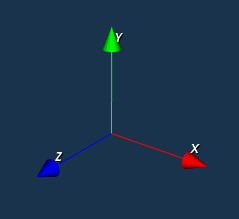
\includegraphics[width=8cm]{imagenes/vtk_axes}
	\caption{Dirección de los ejes XYZ}
	\label{fig:vtk_axes}
\end{figure}

\subsubsection{Visualización}
\begin{itemize}
	\item \textbf{Visualizar en 3D}: Cuando el usuario haya seleccionado una carpeta con datos DICOM, se mostrará en 3D en el widget izquierdo pudiendo rotar y hacer zoom interactuando con el ratón.
	\item \textbf{Visualizar corte}: Cuando el usuario haya cargado los datos DICOM y haya establecido un plano de corte, se podrá generar un corte a la figura por éste. Este corte se visualizará en el widget derecho.
	\item \textbf{Guardar imagen}: El usuario en todo momento podrá guardar una imagen (en formatos comunes JPG o PNG) de lo que está viendo en cada uno de los widgets seleccionando en una ventana que aparecerá cuando se elija la opción la dirección donde se guardará y el nombre del archivo. 
\end{itemize}

\subsubsection{Configuración}
\begin{itemize}
	\item \textbf{Cambiar color de fondo}: El usuario podrá cambiar el color de fondo del widget donde se mostrará la figura en 3D. Para ello podrá:
	\begin{itemize}
		\item Elegir entre colores predeterminados.
		\item Introducir un color mediante valores RGB.
		\item Introducir un color mediante su código de color hexadecimal.
	\end{itemize}
	\item \textbf{Cambiar función de transferencia}: El usuario podrá cambiar la función de transferencia utilizada para poder ver los distintos materiales con una paleta de color distinta a la que se da por defecto.
\end{itemize}

\subsection{Requisitos de rendimiento}

Lala

\subsection{Restricciones de diseño}

Lala

\subsection{Atributos del sistema}

Lala

\subsection{Otros requisitos}

Lala